\begin{figure}[ht!]
    \centering
    % Top figure (full-width)
    \begin{subfigure}{\textwidth} % Full width for the first subfigure
        \centering
        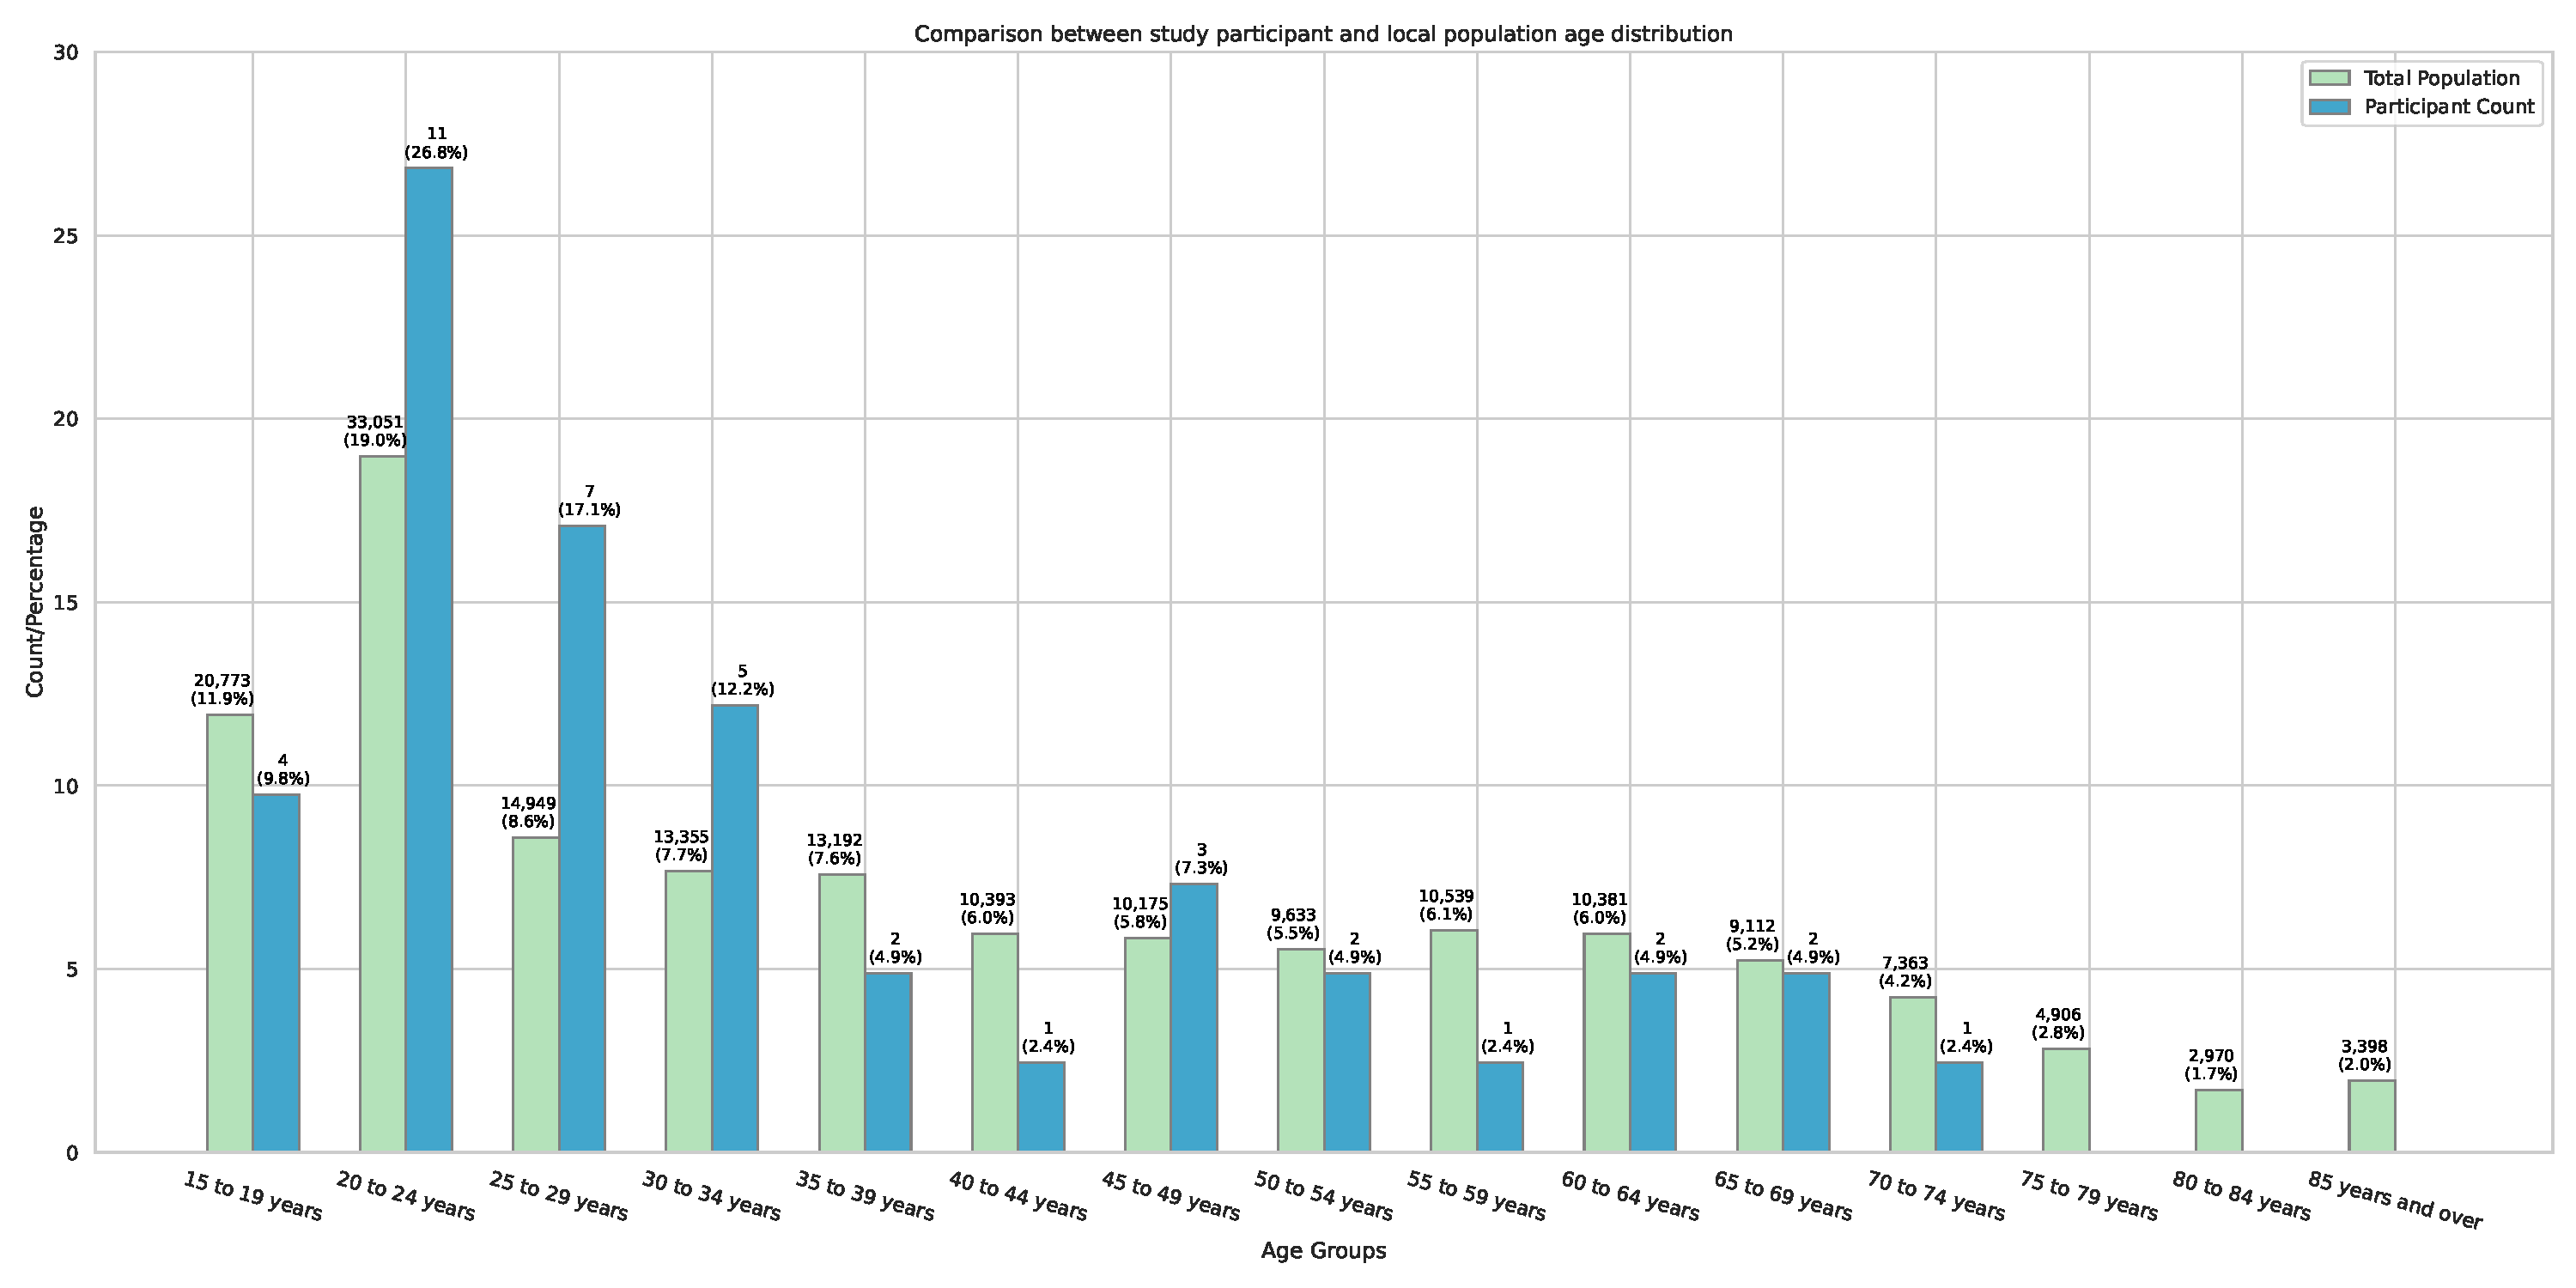
\includegraphics[width=\textwidth, trim=0 13 0 13, clip]{content/image/demo/demo_age_group_vertical.pdf}
        \caption{Age distribution of the study participants were similar to the locale's demographic profile.}
        \Description{A bar chart comparing the age distribution between study participants and the local population. The x-axis represents age groups from 15-19 to 85+, and the y-axis shows count/percentage values ranging from 0 to 30. Each age group has two bars: one for the total population (in peach) and one for participant count (in light blue). Some key differences are visible, such as the 20-24 age group, where the total population is 33,051 (19\%) and participants are 11 (27\%). The 25-29 group shows 14,949 (9\%) for the population and 7 (17\%) for participants. Percentage and count data are displayed above each bar. Other age groups had similar bars. The chart title reads "Comparison between study participant and local population age distribution," and the legend distinguishes the two categories (Total Population and Participant Count).}
        \label{fig:demoAge}
    \end{subfigure}
    
    \vspace{0.25cm} % Add some vertical space between the subfigures

    % Bottom figures (two subfigures side by side)
    \begin{subfigure}{0.45\textwidth} % First subfigure on the second row
        \centering
        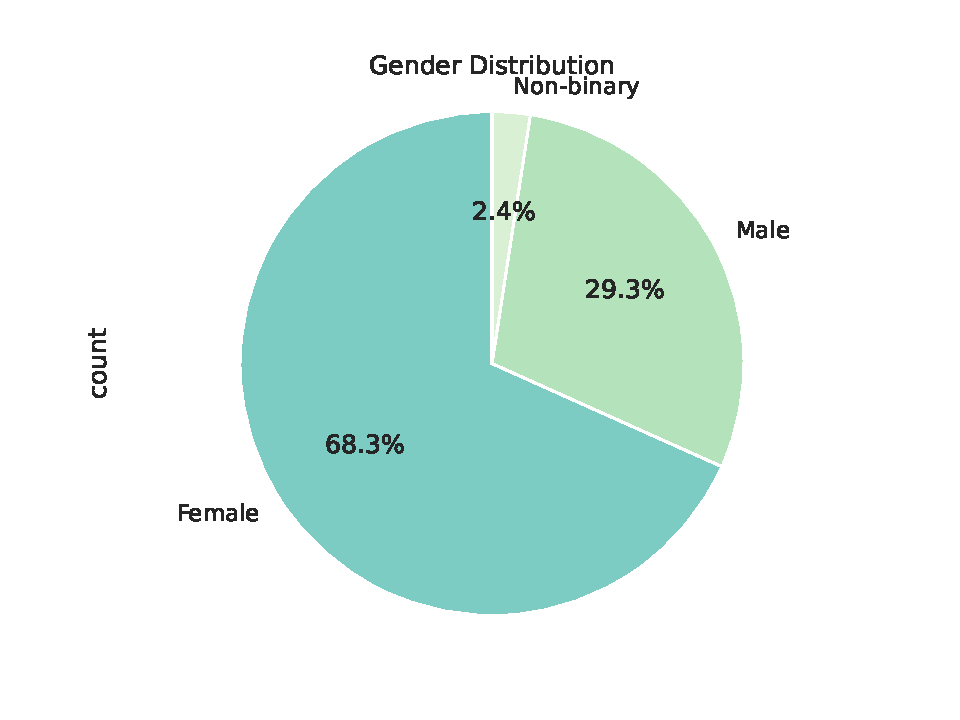
\includegraphics[width=\textwidth]{content/image/demo/demo_gender.pdf}
        \caption{Gender distribution of our participants skewed towards female participants.}
        \Description{A pie chart displaying the gender distribution of study participants. The chart is divided into three sections: 68.3\% (28 participants) are labeled as female and shown in blue, 29.3\% (12 participants) are labeled as male and shown in peach, and 2.4\% (1 participant) are labeled as non-binary, represented by a small gray slice. The title reads "Participant Gender Distribution," and the y-axis on the left is labeled "\% of Participant (Count)."}
        \label{fig:demoGender}
    \end{subfigure}
    \hfill
    \begin{subfigure}{0.45\textwidth} % Second subfigure on the second row
        \centering
        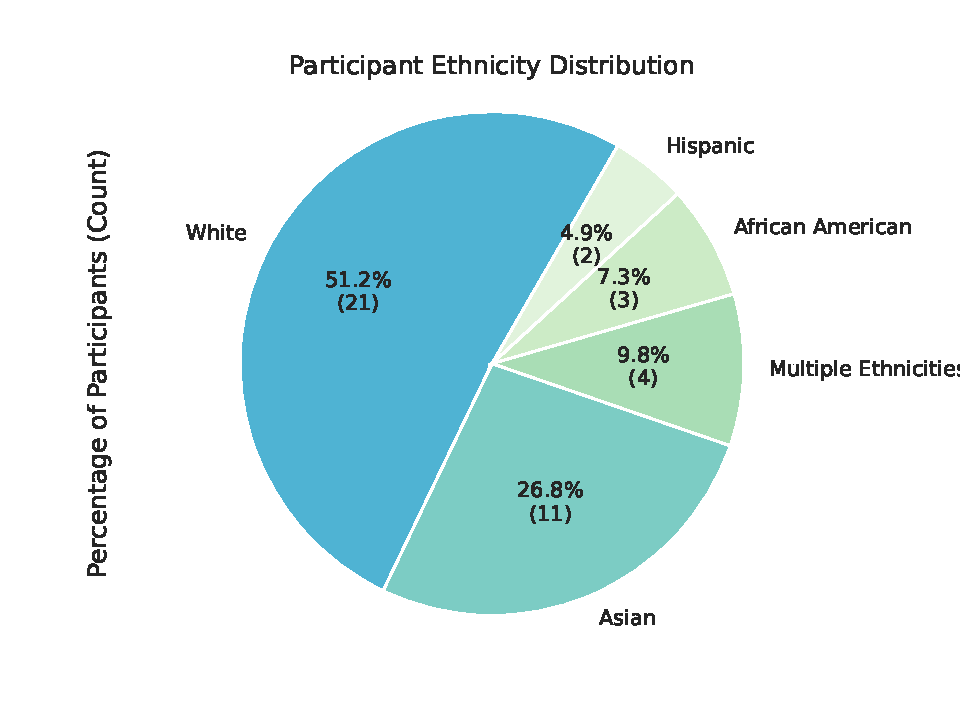
\includegraphics[width=\textwidth]{content/image/demo/demo_ethnicity.pdf}
        \caption{Ethnicity distribution remains diverse with fewer Hispanic and African American participants.}
        \Description{A pie chart showing the ethnicity distribution of participants. The largest segment, representing 51.2\% (21 participants), is labeled White and shown in light blue. Other segments include 26.8\% (11 participants) for Asian, 9.8\% (4 participants) for Multiple Ethnicities, 7.3\% (3 participants) for African American, and 4.9\% (2 participants) for Hispanic. The percentages and counts are displayed within each section. The y-axis on the left is labeled "\% of Participants (Count)," and the title reads "Participant Ethnicity Distribution."}
        \label{fig:demoEthnicity}
    \end{subfigure}

    \caption{Demographic distributions: Age, Gender, and Ethnicity}
    \Description{A collection of three demographic graphs demonstrating age, gender, and ethnicity distribution.}
    \label{fig:Demographics}
\end{figure}


\begin{figure}[ht!]
    \centering
    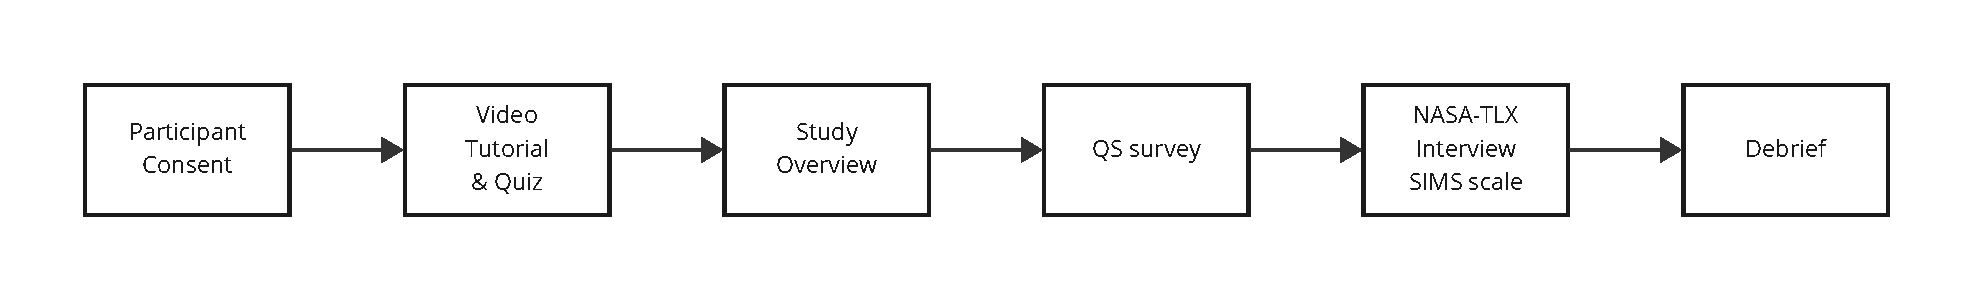
\includegraphics[width=1\textwidth]{content/image/study_flow.pdf}
    \caption{Study protocol: Participants are asked to learn about the mechanism of QS after consenting to the study. The researcher explained the study overview and asked participants to complete the QS. A NASA-TLX survey followed by interviews to understand participants' cognitive load. We debriefed participants after the study.}
    \Description{A flowchart depicting the study protocol, consisting of six stages. Each stage is represented by a rectangular box connected by right-facing arrows. The boxes, from left to right, are labeled: "Participant Consent," "Video Tutorial \& Quiz," "Study Overview," "QS," "NASA-TLX Interview," and "Debrief." The arrows between the boxes indicate the sequence of the study process.}

    \label{fig:studyProtocol}
\end{figure}

\section{Experiment Design}
\label{sec:experiment}
In this section, we describe our experiment design. The study was approved by the university's Institutional Review Board (IRB).

\subsection{Recruitment and Participants}
We recruited 41 participants from a United States college town using online ads, digital bulletins, social media posts, email newsletters, and physical flyers in public spaces beyond campus. We advertised the study as focusing on societal attitudes to mitigate potential response bias. One participant was excluded due to data quality concerns\footnote{The participant reported not completing the survey seriously, as they believed the experiment was fake.}.

To ensure diversity, we prioritized non-students by selectively accepting them and monitoring demographic distribution. The mean participant age was 34.63 years, with an age distribution similar to the county's demographic profile (Figure~\ref{fig:demoAge}), although there was a slightly higher representation of younger adults. Gender and race demographics are presented in Figures~\ref{fig:demoGender} and~\ref{fig:demoEthnicity}. Demographic differences between groups were reasonably balanced, although participants using the short text interface skewed slightly younger ($\mu = 32.1$), and those in the long two-phase interface group had a broader age range ($\mu = 38.8$, $\sigma = 19.6$). Full details are provided in Appendix \ref{sec:apdx:demo}.


\subsection{Experiment Design}
We implemented a between-subject design to minimize fatigue, account for the complexity of QS, and avoid learning effects that could influence participants' cognitive load. The experiment focused on public resource allotment, following the methodology of~\textcite{chengCanShowWhat2021}, in which participants expressed preferences across societal issues. These issues are relevant to all citizens and effectively highlight the need to prioritize limited public resources. Participants received a survey with options randomly drawn from the $26$ societal topics\footnote{See Appendix~\ref{sec:charityList} for the full list.} evaluated by Charity Navigator~\cite{CharityNavigator2023}, an organization that assesses over $20,000$ charities in the United States.
Randomly selecting the options each participant saw aimed to control for potential systematic content biases introduced by specific voting options across surveys of different lengths. Participants were randomly assigned to one of four groups:
\begin{itemize}
    \item Short Text (ST): A text interface with $6$ options. ($N=10$)
    \item Short Two-Phase (SP): A two-phase interface $6$ options. ($N=10$)
    \item Long Text (LT): A text-based interface $24$ options. ($N=10$)
    \item Long Two-Phase (LP): A two-phase interface with $24$ options. ($N=10$)
\end{itemize}

The choice of $6$ and $24$ options, representing short and long lists, was guided by prior research. Studies recommend fewer than 10 options for constant-sum surveys~\cite{moroneyQuestionnaireDesignHow2019} and fewer than 7 for the Analytic Hierarchy Process~\cite{saatyPrinciplesAnalyticHierarchy1987}. Classic cognitive load research~\cite{millerMagicalNumberSeven1956, saaty2003magic} suggests the use of $7\pm2$ items. A meta-analysis by~\textcite{chernevChoiceOverloadConceptual2015} identified $6$ and $24$ as common values for short and long lists in choice overload studies, which are rooted in the original experiment by~\textcite{iyengarWhenChoiceDemotivating2000}.

\subsection{Experiment Procedure}
Participant's spent on average $40$ minutes (min=27, max=68,~$\sigma=9$) in the lab. Figure~\ref{fig:studyProtocol} visually represents the study protocol detailed in the following subsections. 

\subsubsection{Consent, Instructions, and Quiz}
Participants were invited to the lab to control for external influences and used a 32-inch vertical monitor to display all options. After consenting, participants watched a video explaining the quadratic mechanism without any mention of the interface's operation, followed by a quiz to ensure understanding. Participants rewatched the video or consulted the researcher until they successfully selected the correct answers. Each participant's screen was captured throughout the study.

\subsubsection{QS Survey}
The researcher informed participants that the study aimed to help local community organizers understand preferences on societal issues to improve resource allocation. Aware that their screens were being recorded, participants completed the survey independently inside a semi-enclosed space in the lab, without the researcher's presence. Once they completed the survey, participants notified the researcher.

\subsubsection{NASA-TLX Survey and Interview}
The researcher joins study participant with a paper-based weighted NASA Task Load Index (NASA TLX), followed by a semi-structured interview after being informed that the researcher would begin audio recording with their laptop. We adopted the paper-based weighted NASA Task Load Index (NASA TLX), a widely used multidimensional tool that averages six subscale scores to measure overall workload after task completion~\cite{hart1988development, hartNasaTaskLoadIndex2006, cain2007review}. NASA-TLX is favored for its low cost and ease of administration~\cite{gaoMentalWorkloadMeasurement2013}, and it exhibits less variability compared to one-dimensional workload scores~\cite{rubioEvaluationSubjectiveMental2004}, making it suitable for our study. While cognitive load can be assessed through performance, psychophysiological, subjective, and analytical measures~\cite{gaoMentalWorkloadMeasurement2013}, the length and complexity of QS make some of these impractical. Performance and analytical measures require task switching or interruptions, which risk increasing overall cognitive load and experiment time. Psychophysiological measures, such as pupil size~\cite{palinkoEstimatingCognitiveLoad2010} and ECG~\cite{haapalainenPsychophysiologicalMeasuresAssessing2010}, are costly, sensitive to external factors, and often require participants to wear additional equipment.

\subsubsection{Demographic, Debrief, and Compensation}
After the interview, the researcher collected participant's demographics and debriefed them, explaining that the study's goal was to understand interface design and cognitive load. Participants received a \$15 cash compensation.


% performance measures using a secondary task were impractical. Psychophysiological measures such as pupil size~\cite{palinkoEstimatingCognitiveLoad2010} and ECG~\cite{haapalainenPsychophysiologicalMeasuresAssessing2010} were costly and sensitive to external factors. 


 % The complexity of QS survey made completing back-to-back studies impractical. Since preferences are constructed, we wanted to ensure that participants were not influenced by their previous preferences, which could affect their perceived cognitive load and decision-making process.

% asking participants to revisit the lab after several days would likely increase dropout rates and demotivate participants from attending in-person sessions. Second, we aimed to reduce the learning effect, which is challenging to eliminate, especially concerning interface operation and decision-making in the survey. 

% Thus, we adopted these values to align with prior research. \footnote{We believe that the original value decision was due to the limitations of the jam flavors.}

% 

% Therefore, we deployed self-report subjective surveys and analytical measures (i.e., like time and clickstream data). We adopted the paper-based weighted NASA Task Load Index (NASA TLX), a widely used multidimensional tool that averages six subscale scores to represent overall workload after completing a task~\cite{hart1988development, hartNasaTaskLoadIndex2006, cain2007review}. Despite some criticisms, NASA-TLX is favored for its low cost, ease of administration~\cite{gaoMentalWorkloadMeasurement2013}, and significantly less variability compared to one-dimensional workload scores~\cite{rubioEvaluationSubjectiveMental2004}, making it suitable for our study.


% Finally, participants complete the situational motivation scale (SIMS) to gauge motivation and a demographic survey.
% Last, we describe the two quantitative measurements taken during the study: cognitive load and motivation. 
% , indicating differences in workload definitions among raters within a task and variations in workload sources between tasks

% Tabling SIMS for now. It was not used in the analysis. In addition to NASA-TLX, we administered a situational motivation scale (SIMS) to measure participants' motivation (required citation). We posited that motivation would influence mental demand (required citation). SIMS, chosen for its widespread use, helps understand one's intrinsic motivation, extrinsic motivation, identified regulation, and external regulation, and was originally designed to measure self-determination. Both instruments were administered using pen-and-paper.

% The reason we made this experiment design decision was to minimize . External factors, more prevalent in remote experiments or those conducted via platforms like MTurk, included potential multitasking or interruptions by others. An in-lab study also allowed participants to operate across a consistent device that researchers had full control over.